% report.tex

\documentclass[a4paper,11pt]{article}

% Import packages
\usepackage[a4paper]{geometry}
\usepackage[utf8]{inputenc}
\usepackage{amsmath}
\usepackage{amssymb}
\usepackage{graphicx}


% Change enumerate environments you use letters
\renewcommand{\theenumi}{\alph{enumi}}

% Set title, author name and date
\title{Chitty-Chat}
\author{Johannes Jørgensen,} 
\date{\today}

\begin{document} 

\maketitle

\subsection*{Discuss, whether you are going to use server-side streaming, client-side streaming, or bidirectional streaming?}

\subsection*{Describe your system architecture - do you have a server-client architecture, peer-to-peer, or something else?}
\subsection*{Describe what  RPC methods are implemented, of what type, and what messages types are used for communication}
We have implemented a single RPC method called \verb|JoinConversation| that both takes and return a \textit{stream} of type \verb|Message|.
The \verb|Message| type is the message type used for communication. It contains the fields:
\begin{itemize}
    \item \verb|timestamp|: A Lamport timestamp
    \item \verb|username|: The username of the sender
    \item \verb|content|: The content of the message
\end{itemize} 
\subsection*{Describe how you have implemented the calculation of the Lamport timestamps}
Both the server and the client have a \verb|Lamport| clock initilized on start, that is set to \verb|0|. This is also the case for newcomers that connect to the server. 
The \verb|Lamport| clock is handled with these conditions:\\
\textbf{Client:}
\begin{itemize}
    \item When a client sends a message, the \verb|Lamport| clock is incremented by \verb|1|.
    \item When a client receives a message, the \verb|Lamport| clock is incremented by \verb|1| if the timestamp of the received message is greater than the current \verb|Lamport| clock.
\end{itemize}
\textbf{Server:}
\begin{itemize}
    \item When the server receives a message, the \verb|Lamport| clock is incremented by \verb|1| if the timestamp of the received message is greater than the current \verb|Lamport| clock.
    \item When the server broadcasts a message, the \verb|Lamport| will be incremented by \verb|1|.
    \item If a client disconnectes from the server, \verb|Lamport| clock is incremented by \verb|1| - Then the server will broadcast the disconnection.
    \item If a client connects to the server, \verb|Lamport| clock is incremented by \verb|1|- Then the server will broadcast the disconnection.
\end{itemize}
\subsection*{Provide a diagram, that traces a sequence of RPC calls together with the Lamport timestamps}
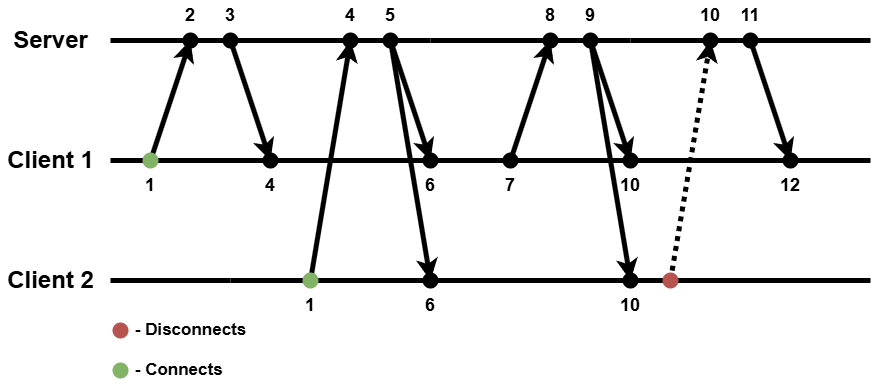
\includegraphics[width=\textwidth]{chat.png}

\subsection*{Provide a link to a Git repo with your source code in the report}
\subsection*{Include system logs, that document the requirements are met, in the appendix of your report}
\subsection*{Include a readme.md file that describes how to run your program.}

\end{document}